%======================================================================
\section{Interface com a rede CAN}\label{sec:can}
%======================================================================
\subsection{O barramento da sala}

A disciplina pede que os módulos de todos os grupos da sala conversem por um barramento CAN.
No nosso sistema, o CAN não é o caminho até a central (isso é o MQTT): ele integra o hub aos
módulos dos outros grupos e publica nele os estados dos sensores do quarto. O vestível também
tem CAN, mas só para bancada e testes; a pulseira de verdade não tem transceptor.

O CAN foi escolhido no primeiro semestre no lugar do RS-485 com Modbus por três motivos que
continuam valendo: o barramento é multimestre, sem um nó que precise perguntar a cada um; a
arbitragem por identificador resolve colisões sem perder a mensagem mais prioritária; e o
controlador do próprio ESP32-S3 faz o enquadramento, o CRC, a confirmação e a retransmissão
em hardware, como define a norma~\cite{iso11898}.

\subsection{Camada física e controlador}

\begin{table}[H]
\centering
\caption{Parâmetros do barramento CAN.}
\label{tab:can_param}
\small
\begin{tabular}{@{}>{\raggedright\arraybackslash}p{3.6cm}>{\raggedright\arraybackslash}p{10.2cm}@{}}
\toprule
Item & Valor \\
\midrule
Controlador & TWAI do ESP32-S3 (compatível com CAN 2.0), TX no GPIO 13 e RX no GPIO 14, nas duas placas \\
Transceptor & SN65HVD230~\cite{sn65hvd230}, de 3,3\,V, no módulo WCMCU-230 (J1), com o barramento em J7 (CANH, CANL, GND) \\
Taxa & 250\,kbit/s \\
Quadro & CAN clássico, identificador padrão de 11 bits, até 8 bytes de dados \\
Terminação & 120\,$\Omega$ nas duas pontas do barramento \\
Filtro de aceitação & em hardware: só os IDs de \code{0x000} a \code{0x0FF} chegam ao firmware \\
Erros & retransmissão até haver confirmação; em \textit{bus-off}, nova tentativa de recuperação com espera de 1 a 60\,s \\
Modo de bancada & autoconfirmação com \textit{loopback} interno, ligado por padrão: testa o firmware sem barramento. Desligado no barramento real \\
\bottomrule
\end{tabular}
\end{table}

O transceptor é de 3,3\,V, o mesmo nível dos GPIOs, e é alimentado pelo regulador da
DevKit; o SN65HVD230 gera os níveis diferenciais do barramento a partir dele. Os pontos de
teste TP5 e TP6, em CANH e CANL, permitem olhar o barramento com o osciloscópio.

\subsection{Identificadores e mensagens}

Toda a identidade de uma mensagem está no identificador, no formato \code{0x0GS}
(Figura~\ref{fig:can_id}): \code{G} é o grupo da sala e \code{S} o sensor dentro do grupo.
Os 8 bytes de dados ficam só para o valor. Esse formato foi combinado entre os grupos: cada
um tem 16 identificadores próprios, e o filtro de hardware descarta o resto. Como no CAN o
menor ID ganha a arbitragem, a prioridade entre os grupos fica definida pelo nibble do grupo.

\begin{figure}[H]
\centering
\resizebox{\linewidth}{!}{% Quadro CAN clássico com ID de 11 bits e o formato 0x0GS do identificador.
\begin{tikzpicture}[font=\scriptsize]
  \tikzset{campo/.style={draw=black!60, fill=#1, minimum height=0.7cm, align=center, inner sep=1pt},
           campo/.default=white}
  % quadro
  \def\y{0}
  \node[campo=black!8, minimum width=0.7cm, anchor=west] (sof) at (0,\y) {SOF\\1};
  \node[campo=corambas!20, minimum width=3.3cm, anchor=west] (id) at (sof.east) {identificador\\11 bits};
  \node[campo=black!8, minimum width=0.7cm, anchor=west] (rtr) at (id.east) {RTR\\1};
  \node[campo=black!8, minimum width=1.0cm, anchor=west] (ide) at (rtr.east) {IDE, r0\\2};
  \node[campo=black!8, minimum width=0.9cm, anchor=west] (dlc) at (ide.east) {DLC\\4};
  \node[campo=corhub!15, minimum width=3.0cm, anchor=west] (dados) at (dlc.east) {dados\\0 a 8 bytes};
  \node[campo=black!8, minimum width=1.2cm, anchor=west] (crc) at (dados.east) {CRC\\15 + 1};
  \node[campo=black!8, minimum width=0.9cm, anchor=west] (ack) at (crc.east) {ACK\\2};
  \node[campo=black!8, minimum width=0.9cm, anchor=west] (eof) at (ack.east) {EOF\\7};
  % zoom do identificador
  \foreach \b [count=\i from 0] in {10,9,8,7,6,5,4,3,2,1,0} {
    \pgfmathsetmacro{\x}{1.0 + \i*0.85}
    \ifnum\b>7 \def\cor{black!8}\else\ifnum\b>3 \def\cor{corambas!30}\else\def\cor{corhub!25}\fi\fi
    \node[campo=\cor, minimum width=0.85cm, minimum height=0.6cm] (b\b) at (\x,-2.0) {\b};
  }
  \draw[decorate, decoration={brace, amplitude=4pt, mirror}] (b10.south west) -- (b8.south east)
       node[midway, below=5pt, align=center] {0\\(ID $\le$ \code{0x0FF})};
  \draw[decorate, decoration={brace, amplitude=4pt, mirror}] (b7.south west) -- (b4.south east)
       node[midway, below=5pt, align=center] {\textbf{G}: grupo\\(\code{0xF} = este projeto)};
  \draw[decorate, decoration={brace, amplitude=4pt, mirror}] (b3.south west) -- (b0.south east)
       node[midway, below=5pt, align=center] {\textbf{S}: sensor\\dentro do grupo};
  \draw[black!40, dashed] (id.south west) -- (b10.north west);
  \draw[black!40, dashed] (id.south east) -- (b0.north east);
  \node[anchor=west, align=left] at (10.6,-2.0) {ex.: \code{0x0F2}\\= grupo F,\\sensor 2 (LM35)};
\end{tikzpicture}
}
\caption{Quadro CAN clássico (campos e número de bits) e o identificador no formato
\code{0x0GS}.}
\label{fig:can_id}
\end{figure}

\begin{table}[H]
\centering
\caption{Mensagens CAN deste projeto (grupo \code{0xF}). Valores em \textit{little endian}.}
\label{tab:can_msgs}
\small
\begin{tabular}{@{}l>{\raggedright\arraybackslash}p{2.1cm}>{\raggedright\arraybackslash}p{2.3cm}>{\raggedright\arraybackslash}p{7.4cm}@{}}
\toprule
ID & Placa & Sensor & Dados \\
\midrule
\code{0x0F1} & hub & HC-SR501 & 1 byte: 0 = livre, 1 = presença \\
\code{0x0F2} & hub & LM35 & 2 bytes: \code{int16} em centésimos de °C \\
\code{0x0F3}--\code{0x0FA} & hub & portas (até 8) & 1 byte: 0 = fechada, 1 = aberta. \code{0x0F3} = quarto, \code{0x0F4} = banheiro \\
\code{0x0FD} & vestível (bancada) & MPU-6050 & 3 bytes: \code{int16} com $\amag^2$ no pico em centésimos de g$^2$ e \code{uint8} com P(queda) em \% \\
\code{0x0FE} & vestível (bancada) & --- & 4 bytes: \code{uint16} bateria em mV (\code{0xFFFF} = não medida) e \code{uint16} atividade em mg \\
\bottomrule
\end{tabular}
\end{table}

O hub envia um quadro a cada mudança de porta ou de presença e a cada leitura de temperatura
(30\,s). Os quadros dos outros grupos e os do vestível em bancada vão para o log do hub; eles
ainda não têm tópico MQTT. Os quadros do vestível não entram nas regras: o alerta de queda
depende do número de sequência do ESP-NOW (Seção~\ref{sec:espnow}).

\paragraph{Carga do barramento.} Um quadro com 1 ou 2 bytes de dados tem cerca de 65 a 75 bits,
contando o enchimento de bits; a 250\,kbit/s, ocupa o barramento por $\sim$0,3\,ms. Mesmo com
as portas e a presença mudando várias vezes por minuto, o hub usa uma fração desprezível do
barramento, que fica para os outros grupos.

\subsection{Implementação}

O componente \code{can} é o mesmo nas duas placas. Qualquer task chama
\code{can\_transmit()}, que só enfileira o quadro; só a task \code{can\_tx} toca o driver.
Assim, nenhuma task espera o barramento, e um barramento sem ninguém (sem confirmação) não
trava quem publica. O estado do nó é acompanhado pela \code{can\_tx}, avisada por notificação:
\begin{itemize}
  \item em \textit{bus-off} (excesso de erros de transmissão), o nó se desliga do barramento,
        como manda o protocolo. O firmware dá \textbf{um} aviso (``CAN sem barramento'') e tenta
        recuperar com espera crescente, de 1 a 60\,s, para não encher o log nem o barramento
        quando ele simplesmente não existe (placa sem transceptor);
  \item só depois que um quadro sai de fato (contador de erros de transmissão zerado) o
        firmware considera o barramento de volta, e avisa uma vez;
  \item quadros que não saem a tempo são descartados, com uma contagem no log.
\end{itemize}

A recepção usa a interrupção do TWAI, que só põe o quadro numa fila; a task \code{can\_rx}
decodifica pelo diretório de identificadores e registra no log. Quadros remotos (RTR) são
ignorados.

\subsection{Validação}

O CAN foi validado com o professor em 28/08/2026, no Projeto 1 deste semestre, com o
firmware de então e os módulos dos outros grupos (Figura~\ref{fig:can_s2p1}). O transporte
foi reescrito depois (filas, recuperação de \textit{bus-off}, diretório de IDs, mapa de pinos
novo), e a versão atual foi verificada em build e no modo de bancada; o teste entre as duas
placas montadas, com transceptores e terminação, está no plano da
Seção~\ref{sec:verificacao}.

\begin{figure}[H]
\centering
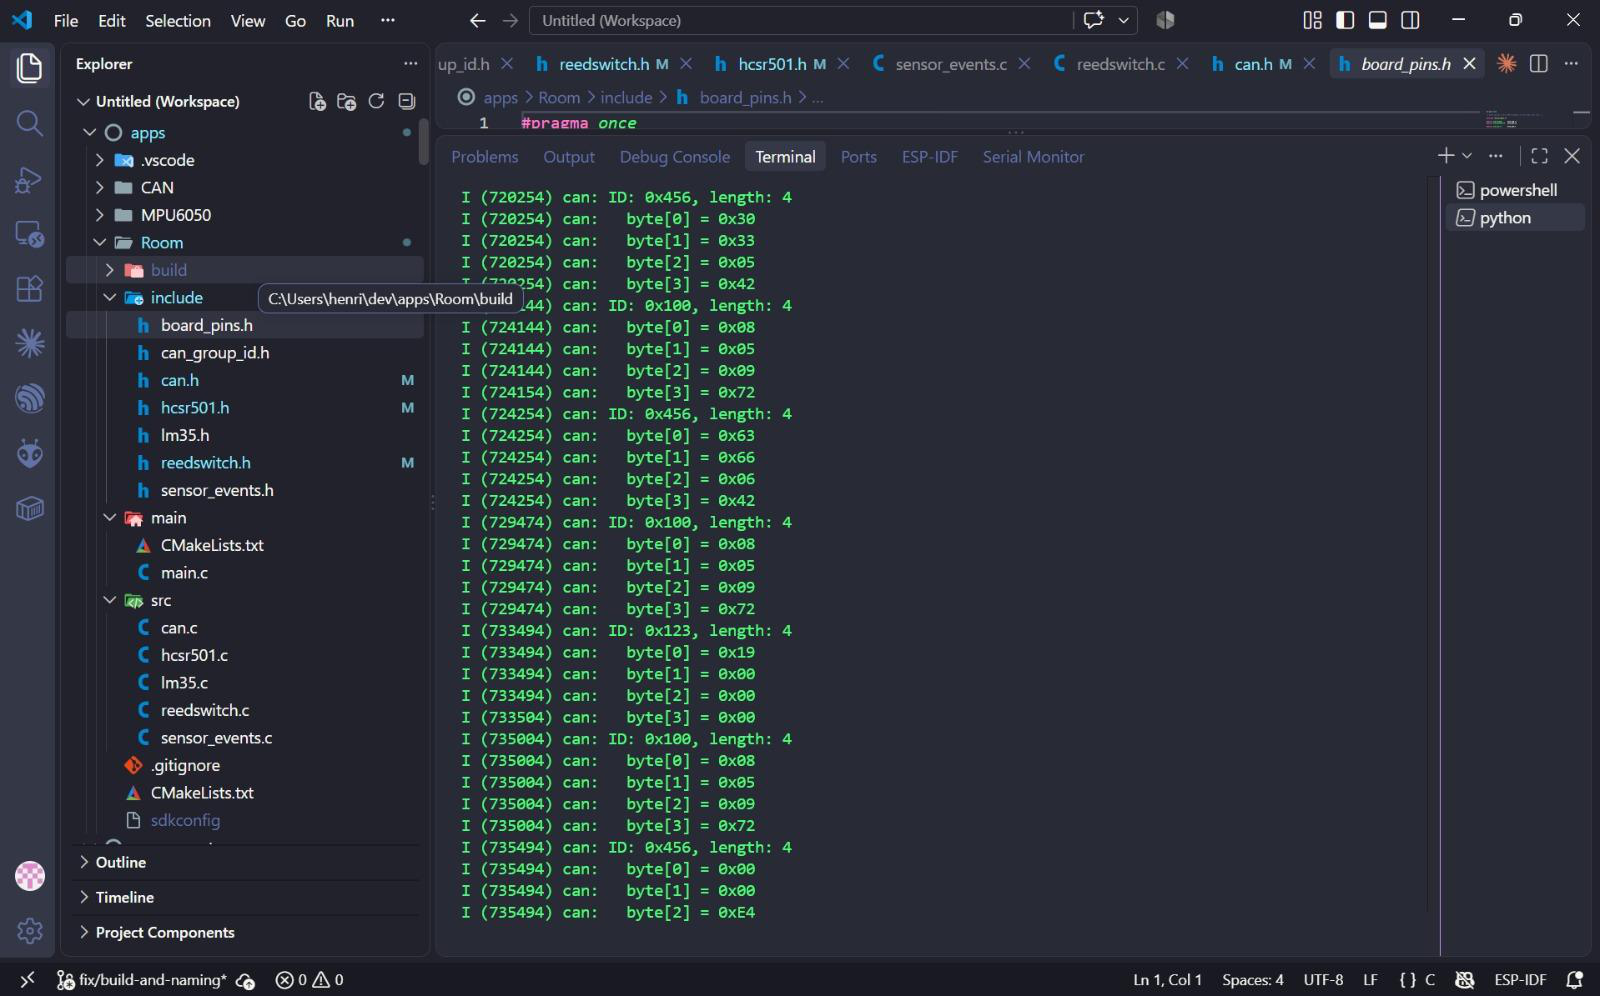
\includegraphics[width=0.85\linewidth]{imagens/s2p1_can_serial.png}
\caption{Monitor serial na validação de 28/08/2026: quadros recebidos do barramento da
sala, com o identificador, o tamanho e os bytes.}
\label{fig:can_s2p1}
\end{figure}

\begin{figure}[H]
\centering
\begin{subfigure}[b]{0.49\linewidth}
  \centering
  \fotoouespaco{bancada_can}{\linewidth}{as duas placas ligadas pelo barramento CAN (transceptores e terminação)}
\end{subfigure}\hfill
\begin{subfigure}[b]{0.49\linewidth}
  \centering
  \fotoouespaco{serial_can}{\linewidth}{monitor serial do hub com os quadros 0x0FD/0x0FE do vestível}
\end{subfigure}
\caption{Teste do CAN entre as duas placas v1.}
\label{fig:bancada_can}
\end{figure}
